The tools used for the benchmark were selected by the capability to determinate 
the presence of the Bufferbloat phenomenon in the network of study by the 
analysis of its indicator, the latency or the round trip time\footnote{To 
SUBTEL, organization responsible for control and supervision in the performance 
of telecommunications in Chile, RTT and Latency correspond to the same thing 
\cite{subtel} }. So, with this as a main consideration, the tool's selected for 
the benchmark will be chosen by the complexity and accuracy to measure and 
determine the RTT into a IP/TCP connection, and how hard is to consistently 
replicate the results under similar contexts. Other tools were selected to help 
to determine to characterize and proof the capability of the network to cause 
Bufferbloat.\\

\newpage 

The tools selected to be used in this tests are the following:

\begin{itemize}
    \item Speedtest test by Ookla
    \item Netalyzr by ICSI
    \item Iperf Tool with Tcptrace/Xplot.org
    \item Page Benchmarker extension for Google Chrome
    \item Smokeping Latency Tool
\end{itemize}

\subsubsection{Speedtest}

Developed by Ookla\footnote{\url{https://www.ookla.com/about}}, this tool is used
for most of the ISPs and many users in Chile to test their broadband's
connections globally. It can be used not only in their website 
\href{http://www.speedtest.net}{\textit{www.speedtest.net}} but also in Android,
iOS or Windows Phone. A command line interface developed in Python can be used 
too for testing Internet bandwidth.\\

The server that will be selected to perform every test, either has or not the
fastest ping, is the one hosted by the Pontificia Universidad Cat\'olica de
Valpara\'iso (this host is the default selected most of times by the site also).  

\subsubsection{Netalyzer}

For end-users, little is revealed about how ISPs manage their networks. That is
why since 2009 ICSI has developed Netalyzr, a ``two click '' tool developed to
test networks that runs in web browser as a Java applet. Once downloaded, the
applet contacts the back-end server using a range of protocols and mechanisms
employed as part of the testing, and then conducts a series of tests. Once
completed, it uploads its findings to the back-end, where they are distilled
into a detailed report breaking down the findings into correctly operating
aspects, those that show potential signs of trouble, and those that are
downright broken. Figure \ref{netaluzr_ex} is an example of the output.\\

\begin{wrapfigure}{r}{0.5\textwidth}
	\begin{center}
		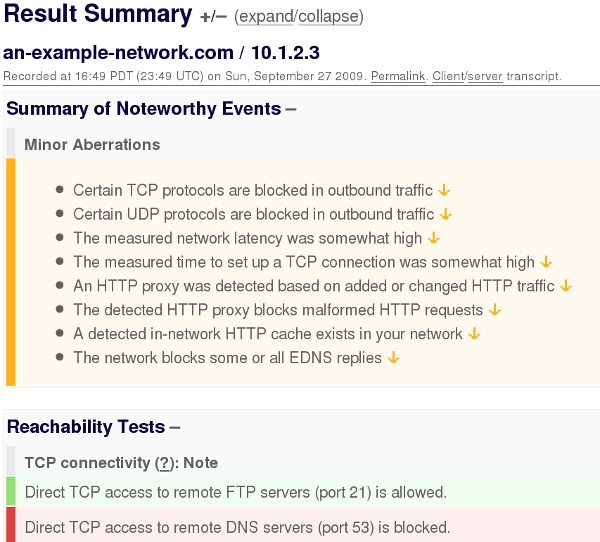
\includegraphics[width=0.48\textwidth]{img/netalyzr_ex}
	\end{center}
	\caption{Result Summary example from Netalyzr. Source:
	\url{www.dslreports.com}}   
	\label{netalyzr_ex} 
\end{wrapfigure}

The primary goal in developing Netalyzr's tests was to provide a new kind of
diagnostic tool, \textit{one that particularly illuminates under what sort of
restrictions a user's Internet connection operates, like both forms of filtering
(blocking) and proxying imposed by the user's ISP, and performance issues that
arise from the nature of the user's Internet access setup}\cite{netalyzr}. Among
the performance considerations, Netalyzr's measure are packet loss, latency,
bandwidth. Also, it compute in-path forwarding device buffer size by comparing
small-packet latencies under idle and loaded states in networks (the perfect
time to occur Bufferbloat). Other tests like general TCP and UDP service
reachability.\\

\subsubsection{Iperf}
Iperf is a well known and commonly used network testing tool. It can create a
TCP and UDP data streams and measure the bandwidth and the quality of a network
link. It can perform multiple tests like Latency, Jitter or Datagram Loss.\\

Iperf basically tries to send as much information down a connection as quickly
as possible reporting on the throughput achieved. This tool is especially useful
in determining the volume of data that links between two machines can supply.
This two machines define the network, one acting like a server and the second as
the client. For this scenario, the server will be the VPS that only will receive
the Iperf connections (also will be running ssh but without further
interaction). The VM Linux machine will work as or Iperf Client.\\  

As mentioned in Iperf users mailing list \textit{
When one runs TCP tests, there are 2 things that block Iperf from having clear
view of real throughput: buffering on sender's side (TCP/IP stack) and TCP
behavior itself (acking). What Iperf can measure is the pace with which it
sends data to TCP/IP stack; TCP/IP stack will only accept data from application
when buffers are not full. If the buffer is huge, Iperf will see high
throughput initially, then it will drop. If there's congestion or retrasmission
going on, Iperf will see it as lower throughput}\cite{iperfmaillist}, but the
data generated by Iperf won't be further analyzed because the  idea behind using
this tool is a TCP's packet generator. This means that the packets generated by 
Iperf will captured and analyzed with tcpdump, tcptrace and xplot.org.\\

\subsubsection{Page Benchmarker}

Page Benchmarker is a Google Chrome extension that intent to test page load 
time performance within Chrome. Measures time-to-first-paint, overall page load 
time KB read/written, and several other metrics, and with its capability to 
clear the cache and existing connections between each page load, makes this 
tool one of the main sources results.\\

\subsubsection{Smokeping}
SmokePing is a latency logging and graphing tool that consists of a running 
daemon which organizes the latency measurements and a CGI which presents the 
graphs. With SmokePing give us the ability to measure latency and packet loss 
in the current network, with RRDtool is capable to maintain a long term 
data store and to draw different graphs with the giving up to the minute 
information on the state of each network connection.\\

Smokeping can be configured to perform a wide range of latency measurement 
probes each one directed to an independent target or over a set of targets 
selected for each proof.\\
